\documentclass[margin,line]{CV}

\usepackage{graphicx}
\usepackage{wrapfig}
\usepackage{ifthen}
\usepackage{hyperref}

\newboolean{foreign}
\setboolean{foreign}{false}

%\def\superofficial{}
\def\consentclause{}

\begin{document}
\name{\Large Alexander Fokin}
\begin{resume}

%\begin{wrapfigure}{r}{2cm}
%    \vspace{-20pt}
%    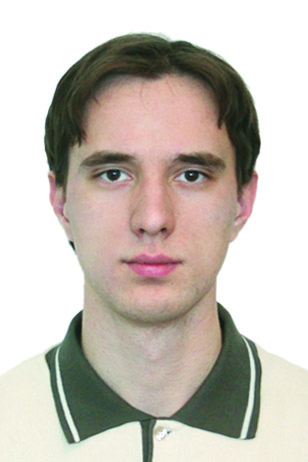
\includegraphics[width=2cm]{photo.jpg}
%    \vspace{-20pt}
%\end{wrapfigure}

    \section{\mysidestyle Contact\\Information}
    Telegram (preferred): \href{https://t.me/fokin_alexander}{@fokin\_alexander} \\
    E-mail: apfokin@gmail.com \\
    LinkedIn: \url{https://linkedin.com/in/apfokin} \\
    %Current location: Frankfurt, Germany

    \section{\mysidestyle Professional\\Experience}
    \textbf{ISO C++ Standards Committee}\vspace{1mm}\\
    \textsl{C++ Expert} \hfill \textbf{May 2016 - present}\vspace{1mm}\\
    Started WG21 Russia in 2016 and currently representing the Russian national body in the ISO C++ standards committee. I have some of my code in the standard, and I have been giving talks and hosting C++ events since 2015.

\ifdefined\superofficial
    {\footnotesize\textit{ISO C++ Standards Committee is called WG21, officially ISO/IEC JTC1 (Joint Technical Committee 1) / SC22 (Subcommittee 22) / WG21 (Working Group 21). More info is available at \url{http://isocpp.org} and \url{http://stdcpp.ru}.}}
\fi


    \vspace{2mm}
    \textbf{Ozon}, Moscow, Russian Federation\vspace{1mm}\\
    \textsl{Director, Search \& Platform} \hfill \textbf{October 2019 - January 2022}\vspace{1mm}\\
    Joined Ozon at a turbulent time when it was growing over 100\% YoY. 

    Was responsible for all of Ozon infrastructure, from the datacenter level, all the way up to common libraries used throughout the company. Was handed the teams when the previous CTO has left the company, so was tackling a lot of hard problems at the same time --- scaling the infrastructure to meet business needs, doing the reorgs necessary, limiting the damage from people following in the previous CTO's footsteps, hiring like crazy, both into IC and leadership positions, and making technical decisions myself when the teams lacked the necessary skills or perspective.

    Was also responsible for all of machine learning / data science efforts in the company, including search quality, personal recommendations, antifraud, demand prediction, automatic moderation and SKU matching.  Dealt away with the matrix structure that made it hard for the ML teams to actually focus on the product, was hiring non-stop, and was helping the teams with product vision and technical decisions.

    In terms of product teams, was leading market monitoring and search \& recommendations. For my last year at Ozon was mainly focusing on search, driving a number of projects on all levels of the search stack:
    \begin{itemize}
    \item Implementing a custom search engine based on Apache Lucene, bringing significant performace gains. At 2021 peaks we were handling over 10K RPS for a continuously updating search index of 10s of millions of SKUs.
    \item Implementing a custom realtime personal recommendations engine.
    \item Shipping a unified system for A/B test analysis that was subsequently used all throughout the company.
    \item Designing and implementing several different advertising formats in search and recommendations, positively affecting the company's EBITDA. This was very successful, to the point that competitors started rolling out the same formats several months after our launch.
    \item Continuously improving search and recommendations quality.
    \end{itemize}
    %\vspace{-4mm}
    
    In terms of the tech stack, my teams were using a variety of languages, including Go, Java, C\# and Python. On the infrastructure side we were using pretty much everything that the opensource world has to offer, including K8s, PostgreSQL, Redis, ClickHouse, Hadoop, etc.

    \vspace{2mm}
    \textbf{Yandex}, Moscow, Russian Federation\vspace{1mm}\\
    \textsl{Head of Search Components \& Safe Search} \hfill \textbf{June 2019 - October 2019}\vspace{1mm}\\
    \textsl{Head of Search Components} \hfill \textbf{October 2015 - June 2019}\vspace{1mm}\\
    \textsl{Senior Search Engineer} \hfill \textbf{October 2014 - October 2015}\vspace{1mm}\\
    Was responsible for Yandex web search runtime, antispam / safe search, and parts of internal cloud infrastructure, managing a team of over 100 engineers.
    
    \pagebreak

    The most important projects that I have worked on are as follows:
    
    \begin{itemize}
    \item Redesigning the search stack for the modern times of cheap SSDs, fast networks, and DSSMs. Over the years pretty much everything about the search stack was changed, even including how it was split into services. I wrote most of the foundational code for the first step in this process, squeezing out as much performance as possible by using all of the low-level tricks known to humanity and consulting with our linux kernel engineers, and throughout the next several years we continued to ship incremental improvements, getting the number of document in the search index to 100s of billions while simultaneously bringing substantial performance and quality gains.
    \item Improving technical interviews in the company, making them standardized and consistent. This was a company-wide project that has included everything from researching how it's done in other companies, to doing lectures on best interviewing practices, preparing 100s of interviewers, creating an online seminar, incrementally improving the rules, and scaling it all up when I was no longer able to do everything by myself. This basically amounted to single-handedly turning a ship of over 4000 developers 90 degrees while all of them protested, and in terms of long-term impact on the company this was likely the most important effort that I led at Yandex.
    \item Revitalizing the codebase and creating a system that would motivate developers to pay off technical debt in common code. This was also a company-wide project that started with me porting clang's libcxx to MSVC so that we could switch to C++11 STL, and realizing that this effort could be crowdsourced. This then paved way to some important repository-wide refactorings that would not have been possible otherwise.
    \end{itemize}
    \vspace{-4mm}

    In terms of the tech stack, I was mostly writing C++ code, and my teams were using either C++ or Python. On the infrastructure side pretty much everything used at Yandex is developed in-house.

\ifdefined\superofficial
    {\footnotesize\textit{Yandex is one of the largest internet companies in Europe, operating Russia's most popular search engine. More info is available at \url{https://yandex.com/company/}.}}
\fi 


    \vspace{2mm}
    \textbf{Network Optix}, Moscow, Russian Federation, then Los Angeles, USA\vspace{1mm}\\
    \textsl{Senior Software Engineer} \hfill \textbf{October 2011 - July 2014}\vspace{1mm}\\ 
    Designed and implemented initial version of the Nx Witness client application, making sure that its high-level architecture is sound and extensible.

    As the person solely responsible for the client-facing part of the system, I made no compromises when it came to delivering the best experience for the users. After 1.0 release various sources have described Nx Witness as the most user-friendly and aesthetically pleasing video management system on the market, which has helped the company to gain a competitive edge.

    Was subsequently charged with management of the front-end development team. Other responsibilities included design of public APIs and development of generic C++ libraries that were used internally.
    
\ifdefined\superofficial
    {\footnotesize\textit{Network Optix is an enterprise video software development company headquartered in Burbank, CA, focused on building easy-to-use video management technologies. More info is available at \url{http://www.networkoptix.com/}.}}
\fi
    
    
    \vspace{2mm}    
    \textbf{SmartDec}, Moscow, Russian Federation\vspace{1mm}\\
    \textsl{Software Engineer} \hfill \textbf{July 2009 - September 2011}\vspace{1mm}\\
    Was mainly working on SmartDec, a native code decompiler. Laid out the architecture of the decompiler and implemented several frontend and backend plugins, including support for different x86 and PIC assembly input formats. Was responsible for devising novel algorithms that would improve the quality of the decompiled code and would allow for reconstruction of C++-specific constructs. This effort has led to several publications on international conferences on reverse engineering.

    Have also implemented a form recognition toolkit that was subsequently used in some of the Moscow schools for test checking. 
    %Detailed description is available at \url{http://elric.ru/wordpress/projects/form-recognition-toolkit/}. 

    %Was additionally working on \url{http://mathege.ru}, a national mathematics exam portal. Did both frontend and backend development and have implemented a \LaTeX~to html converter that was used for importing problems into the system.

\ifdefined\superofficial
    {\footnotesize\textit{SmartDec is a software security consulting company specializing in vulnerability analysis and reverse engineering. More info is available at \url{http://smartdec.net}.}}
\fi
    
    
    \vspace{2mm}
    \textbf{Institute for System Programming of the Russian Academy of Sciences}, Moscow, Russian Federation\vspace{1mm}\\
    \textsl{Software Engineer} \hfill \textbf{September 2007 - September 2008}\vspace{1mm}\\
    Was working in a team developing a framework for dynamic analysis of binary code and implemented a disassembler for MIPS64 architecture that significantly outperformed all other disassemblers for this architecture.

\ifdefined\superofficial
    {\footnotesize\textit{ISPRAS is an R\&D organization in the field of system programming and software engineering. Among its clients are leading IT companies such as HP, IBM, Intel and others. More info is available at \url{http://www.ispras.ru/en/}.}}
\fi
    
    \pagebreak

    \vspace{2mm}
    \textbf{Intel}, Moscow, Russian Federation\vspace{1mm}\\
    \textsl{Software Engineering Intern} \hfill \textbf{February 2007 - April 2008}\vspace{1mm}\\
    Was researching computer vision algorithms and have implemented a panorama stitching application. Was also charged with the development of Ruby bindings for Intel's Integrated Performance Primitives library.
    
\ifdefined\superofficial
    {\footnotesize\textit{Intel is an American multinational corporation and technology company. More info is available at \url{http://www.intel.com}.}}
\fi
    
   
    \section{\mysidestyle Education}
    \textbf{Department of Computational Mathematics and Cybernetics, Moscow State University}, Moscow, Russian Federation\vspace{1mm}\\
    \textsl{\ifthenelse{\boolean{foreign}}{Bachelor's}{Specialist} degree in Applied Mathematics and Computer Science} \hfill \textbf{September 2004 - July 2009}\vspace{1mm}\\
    Advisor: Professor Alexander Chernov \\
    Thesis: Reconstruction of Class Hierarchies for Decompilation of C++ Programs \\
    Graduated with high honors. Diploma GPA is 5.0 out of 5.0.

    \textbf{Graduate School of Science and Engineering, Chuo University}, Tokyo, Japan\vspace{1mm}\\
    \textsl{Full-time non-degree student} \hfill \textbf{September 2008 - March 2009}\vspace{1mm}\\
    Advisor: Professor Mitsunori Makino \\
    Was studying Japanese, working on algorithms for real-time ray tracing and implemented a real-time ray tracer for use with CAVE automatic virtual environment.

    
    \section{\mysidestyle Publications}
    A. Fokin, E. Derevenetc, A. Chernov and K. Troshina. ``SmartDec: Approaching C++ Decompilation'',
    in proceedings of the \textsl{18th Working Conference on Reverse Engineering}, pp. 347-356, 2011.

    A. Fokin, K. Troshina and A. Chernov. ``Reconstruction of Class Hierarchies for Decompilation of C++ Programs'',
    in proceedings of the \textsl{14th European Conference on Software Maintenance and Reengineering}, pp. 249-252, 2010.

    K. Troshina, A. Chernov and A. Fokin. ``Profile-Based Type Reconstruction for Decompilation'',
    in proceedings of the \textsl{17th International Conference on Program Comprehension}, pp. 263-267, 2009.


%    \section{\mysidestyle Honours, \\Awards and \\Test Scores}
%    TOEFL iBT, 111/120, Moscow, 2010.                                                               \vspace{1mm}\\
%    M.V. Lomonosov Scholarship for Academic Excellence, Moscow, 2006-2009.                          \vspace{1mm}\\
%    ABBYY Collegiate Mathematics Competition, 1st place, Moscow, 2006.                              \vspace{1mm}\\
%    8th Moscow Collegiate Programming Contest, 9th place, Moscow, 2006.                             \vspace{1mm}\\
%    7th Moscow Collegiate Programming Contest, 11th place, Moscow, 2005.                            \vspace{1mm}\\
%    Unified State Exam in Mathematics, 100/100 (nationwide top), Izhevsk, 2004.                     \vspace{1mm}

%    \section{\mysidestyle Professional\\Skills}
%    Programming Languages: substantial experience with C++ and Java; experience with Delphi, x86 Assembly; some experience with C\#, Matlab, Perl and Python. \\
%    Libraries and Framewords: considerable experience with modern C++ libraries and frameworks such as Qt and boost. \\
%    Platforms: Windows, Linux, Mac OS X. A lot of experience writing cross-platform code. \\
%    Databases: MySQL, SQLite.

    \section{\mysidestyle Languages}
    Russian: native. \\
    English: fluent. \\
    Japanese: elementary.
  
    \ifdefined\consentclause
    \vspace{5mm}
    {\footnotesize\textit{I hereby give consent for my personal data included in my application to be processed for the purposes of the recruitment process under the Personal Data Protection Act as of 29 August 1997, consolidated text: Journal of Laws 2016, item 922 as amended.}}
    \fi
    
    
\end{resume}
\end{document}



















